%%
%% This is file `sample-sigchi.tex',
%% generated with the docstrip utility.
%% but modified by the faculty @ DI/FCUL
%% The original source files were:
%%
%% samples.dtx  (with options: `sigchi')
%% 
%% IMPORTANT NOTICE:
%% 
%% For the copyright see the source file.
%% 
%% Any modified versions of this file must be renamed
%% with new filenames distinct from sample-sigchi.tex.
%% 
%% For distribution of the original source see the terms
%% for copying and modification in the file samples.dtx.
%% 
%% This generated file may be distributed as long as the
%% original source files, as listed above, are part of the
%% same distribution. (The sources need not necessarily be
%% in the same archive or directory.)
%%
%% The first command in your LaTeX source must be the \documentclass command.
\documentclass[sigplan]{acmart}
\settopmatter{printacmref=false} % Removes citation information below abstract
\renewcommand\footnotetextcopyrightpermission[1]{} % removes footnote with conference information in first column
\usepackage{subcaption}
\usepackage{caption}
\usepackage{array}
\usepackage{multirow}
\usepackage{listings}
\usepackage{mathpartir}
\usepackage{bussproofs}
\usepackage{amssymb}
\usepackage{stmaryrd}
\usepackage{tikz}
\usetikzlibrary{matrix}

\lstset{basicstyle=\small, mathescape=true, language=Haskell}  

\newcommand{\srule}[1]{\textsc{#1}}


%% end of the preamble, start of the body of the document source.
\begin{document}

\title{Type Operators in FreeST} 

\author{Paula Inês Garcias Lopes - 60900}
\affiliation{%
 \institution{
  Estudo Orientado \\ 
  Mestrado em \{Engenharia Informática\} \\ 
  Faculdade de Ciências, Universidade de Lisboa}
 }
\email{fc60900@fc.ul.pt}


\begin{abstract}
  In this work we study system $F^{\mu;}_\omega$, the higher-order polymorphic lambda calculus equipped with equirecursive and context-free session types, as well as its seamless integration into FreeST, a functional programming language governed by context-free session types. We talk about the hardships of finding practical type equivalence algorithms that can be implemented into programming languages compilers, describe a possible algorithm for FreeST and define some guidelines for the work to follow.
\end{abstract}


%%
%% Keywords. The author(s) should pick words that accurately describe
%% the work being presented. Separate the keywords with commas.
\keywords{FreeST, Higher-order Kinds, Context-free Session Types}

\pagestyle{plain} % removes running headers

%%
%% This command processes the author and affiliation and title
%% information and builds the first part of the formatted document.
\maketitle
\section{Introduction} \label{sec:intro}

Exploring sophisticated type systems and their seamless integration into programming languages is a thoroughly researched field. System $F^\mu$ \cite{GauthierP04} up to System $F^\mu_\omega$ \cite{DBLP:conf/popl/CaiGO16}, how far can we go until these systems are no longer suitable for compilers.\\

FreeST \cite{AlmeidaMTV22}, a functional programming language based on system $F^{\mu;}$, is regulated by context-free session types. The current type equivalence algorithm in FreeST was developed by Almeida et al. \cite{AlmeidaMV20}. The next step is to elevate it to a higher-order setting, which is the goal of this work.\\

\textit{Beyond first-order context-free session types.   }  
The recursive type $\mu\alpha\colon S.\&\{Leaf\colon Skip,\  Node\colon\alpha;?Int;\alpha\};Close$ describes a protocol for safely streaming integer trees on channels. If the continuation of the channel is $Leaf$, then no communication occurs but the channel is still open for further composition whereas, if the continuation of the channel is $Node$, then we have the left subtree, an integer and a right side subtree. When the whole tree is received, the channel is closed.
Instead, we are interested in abstracting the type that is received on the tree channel, $\mu\alpha\colon T.\mu\beta\colon S.\&\{Leaf\colon Skip,\\
Node\colon\beta; ?\alpha; \beta\};Close$, by using higher-order kinds, that is, type operators.\\

\textit{Type checking algorithms for compilers.  }
We desire a powerful type system with vast expressiveness. However, expressive type systems pose threats to the compilers of the habitat where they live: programming languages. Necessarily, analysing the type equivalence problem is a top priority. It is common knowledge that the type equivalence of context-free session types is decidable, but for higher-order context-free session types it may no longer be. Ultimately, the measure of decidability alone is not sufficiently valuable. We are interested in practical algorithms for type equivalence checking to be incorporated into compilers. Therefore, another goal of this work is to better analyse the limitations of type equivalence algorithms.\\

\textit{Duality as an external macro (or not).   }
Usually, duality is offered as a built in constructor \cite{DBLP:journals/corr/abs-2004-01322}. However, we believe duality should be internal, a type operator. We plan to internalise the $Dual$ type operator in FreeST by allowing higher-order polymorphism.\\

\textit{Outline. } 
The rest of the paper is organised as follows: Section 2 sums up important notions for a better understanding of our work; Section 3 describes related work; Section 4 introduces System $F^{\mu;}_\omega$ and type equivalence; Section 5 demonstrates a small example that benefits from types $F^{\mu;}_\omega$; Section 6 wraps up the paper, providing directions for future work.

\section{Background} \label{sec:background}
Within this section we include relevant definitions essential for a thorough understanding of our work. 

\paragraph{Substitution.}
Firstly, the notion of substitution. In lambda calculus \cite{Church1936AnUP}, substitution replaces all free occurrences of a variable in a expression with another expression, written as $[x \rightarrow E_1]E_2$. We use this concept as well as the notion of free variables, $\mathit fv(x)$, later when describing our work.

\paragraph{Kinds and Type operators.}
In programming languages, values are categorized by types, while kinds play the role of categorizing these types. A kind can be built from the kind $\star$ and constructor $\Rightarrow$. We have:

\begin{itemize}
    \item $\star$ the kind of proper types;
    \item $\star\Rightarrow\star$ the kind of type operators;
    \item $\star\Rightarrow(\star\Rightarrow\star)$ the kind of functions from proper types to type operators;
    \item $(\star\Rightarrow\star)\Rightarrow\star$ the kind of functions from type operators to proper types;
\end{itemize}

Note that proper types refers to types that classify values and are well-formed, such as integers, booleans,  term-level abstractions. In contrast, type operators are type constructors; they operate at the level of types and can be used to create more complex types. For example, the type operator $(\rightarrow)$ takes two types, one on the left side and one on the right side of the arrow and constructs a new type, a function type $a \rightarrow b$.

All proper types belong to kind $\star$ whereas type operators belong to the kind $\star\Rightarrow\star$. Also, just like some values don't have a type, any ill-formed type has no kind.
This is the core notion of our work. It is our intention to expand the programming language FreeST, currently limited to kind $\star$, to higher-order types.

\paragraph{Simple Grammars.}
Following Almeida's algorithm et al. \cite{AlmeidaMV20}, the approach chosen for checking type equivalence involves reducing the problem to checking the bisimilarity of simple grammars.\\
Grammars can be specified by tuples of the form $(\mathcal{T, N}, X, \mathcal{R})$. 
\begin{enumerate}
    \item $\mathcal{T}$ is a finite set of terminal symbols such as $a, b, c$; 
    \item $\mathcal{N}$ is a finite set of non-terminal symbols, $X, Y, Z$;
    \item $X$ is the starting symbol. $X$ must be an element of $\mathcal{N}$, $X\in\mathcal{N}$;
    \item $\mathcal{R}$ is a finite set of productions, where $P \subseteq N \times (T \cup N)^*$. 
\end{enumerate}
A production rule in $\mathcal{R}$ is written as $X \rightarrow \sigma$: the left side of the arrow must be a non-terminal, $X\in\mathcal{N}$, while the right side must be a word, such that $\sigma\in(\mathcal{N}\cup\mathcal{T})^*$. Also, $\sigma$ can be the empty word.

We are particularly interested in simple grammars in Grei-bach normal form \cite{AutebertG84}. Grammars are in Greibach normal form if production rules take form as $X \rightarrow a\gamma$, where $X\in\mathcal{N}$, $a\in\mathcal{T}$ and $\gamma\in\mathcal{N}^*$. Grammars in GNF are \emph{simple} when for every non-terminal and terminal symbol there is at most one production $X \rightarrow a\gamma$ \cite{KorenjakH66}.

The notion of simple grammars will be important when discussing our type equivalence algorithm and its decidability later in section \ref{sec:typeop}.

\section{Related Work} \label{sec:relatedwork}
Briefly, we explore work akin to ours.\\

\textit{Session type systems.   }
The inception of session types dates back to the 1990s \cite{Honda93, HondaVK98, TakeuchiHK94}. Context-free session types arose from the aspiration to expand session type theory to non-regular protocols \cite{Puntigam99,RavaraV97}.

A type system's value is directly tied to its feasibility within a programming language. The inclusion of context-free session types augments the expressiveness and adaptability of communication protocols in programming languages.

FreeST \cite{AlmeidaMTV22, freest} is a concurrent functional programming language equipped with context-free session types. By taking advantage of a process algebra graph representation of types to decide bisimulation, Almeida et al. \cite{AlmeidaMV20} developed an algorithm to decide the equivalence of context-free session types.

Padovani \cite{DBLP:journals/toplas/Padovani19} introduces a language with context-free session types that avoid the problem of checking type equivalence by requiring annotations in the source code.\\

\textit{Type equivalence algorithms.    }
Algorithms for deciding the equivalence of types are intricately tied to the computational power and expressiveness of the underlying type system: the more expressive the type system is, the more sophisticated the algorithm will be.

Thiemann and Vasconcelos proved that type equivalence of context-free session types is decidable \cite{ThiemannV16} by reducing the problem to the verification of bisimulation for Basic Process Algebra (BPA). Most works about the decidability of the equivalence of BPA terms provide no immediate practical algorithm, except the work by Czerwiński and Lasota \cite{CzerwinskiL10} where a polynomial time algorithm is presented. However, their work focuses on the bisimilarity of normed context-free processes and context-free session types are not necessarily normed. 

Almeida's algorithm et al. \cite{AlmeidaMV20} decides the equivalence of context-free session types by reducing the problem to the bisimilarity of simple grammars. Baeten \cite{BaetenBK93} proved the equivalence between grammars in Greibach form and BPA processes.

\section{System $F^{\mu;}_\omega$} \label{sec:typeop}
This section introduces the meta-theory of System $F^{\mu;}_\omega$ as well as describe our work.

\subsection{Kinds, Types and Type formation}
Distinguishing between session and functional types is achie-
ved by categorizing them as kinds $S$ and $T$, respectively; $\star$ denotes the kind of proper types, while $\kappa$ represents either the kind of proper types or type operators, $\kappa\Rightarrow\kappa'$.
\begin{align*}
  \mathtt \star ::= & & \textit{Kind of proper types}\\
  & \mathtt S & \textit{session}\\
  & \mathtt T & \textit{functional}\\
  \mathtt \kappa ::= && \textit{Kind}\\
  & \mathtt \star & \textit{kind of proper types}\\
  & \mathtt \kappa \Rightarrow \kappa & \textit{kind of type operators}
\end{align*}

A type is either a constant $\iota$, a type variable $\alpha$, an abstraction $\lambda\alpha\colon\kappa.T$ or an application $T U$. A type constant is either an arrow, record or variant, recursive type, universal type, skip, wait and close, sequential composition, choice operators, intput/output operators, or the dual operator.

% Type operators and Types %
\begin{align*}
  \mathtt \iota :: = & & \textit{Type constant}\\
  & \mathtt \rightarrow & \textit{arrow}\\
  & \mathtt {\llparenthesis\overline{l_i}\rrparenthesis} & \textit{record, variant}\\
  & \mathtt \mu_\kappa & \textit{recursive type}\\
  & \mathtt \forall_\kappa & \textit{universal type}\\
  & \mathit{Skip} & \textit{skip}\\
  & \mathit{Wait} & \textit{wait}\\
  & \mathit{Close} & \textit{close}\\
  & \mathtt \# & \textit{input, output}\\
  & \mathtt ; & \textit{sequential composition}\\
  & \mathtt \odot \{\overline{l_i}\} & \textit{choice operator}\\
  & \mathit{Dual} & \textit{dual operator}\\
  & \mathtt () & \textit{unit type}\\
  \mathtt T ::= && \textit{Type}\\
  & \mathtt \iota & \textit{type constant}\\
  & \mathtt \alpha & \textit{variable}\\
  & \mathtt \lambda\alpha\colon\kappa.T & \textit{type-level abstraction}\\
  & \mathtt {T T} & \textit{type-level application}
\end{align*}
\vspace{3mm}

Subsequently, we present a few notions before reaching the main result of this section, type formation.

\textit{Renaming.    } 
Taking inspiration from the notion of renaming from Gauthier and Pottier \cite{GauthierP04}, the definition of type renaming is as follows:


$$
\begin{aligned}
\operatorname{rename}_{S}(\iota) = &\ \iota \\
\operatorname{rename}_{S}(\alpha) = &\ \alpha \\
\operatorname{rename}_{S}(\lambda\alpha\colon\kappa . T) =  &\ \lambda v\colon\kappa . \operatorname{rename}_{S}(T[v / \alpha]) \\
 & \quad\quad \text { where } v=\operatorname{first}_{S}(\lambda\alpha\colon\kappa . T) \\
\operatorname{rename}_{S}(T U) = &\ \operatorname{rename}_{S \cup\operatorname{fv}(U)}(T) \operatorname{rename}_{S}(U)
\end{aligned}
$$
\vspace{3mm}

Renaming consists on replacing a type $T$ by a minimal alpha-conversion of itself. This means we rename bound variables in $T$ by the smallest possible variable available. We assume a countable ordered set of type variables, $\{ v_1, .., v_n ... \}$, available for renaming. Therefore, there will always be at least one type variable available for renaming.
Note that the $S$ parameter is the set of unavailable type variables for renaming.  Also, by $\operatorname{first}_{S}(\lambda\alpha\colon\kappa.T)$ we mean the smallest variable not in set $S\cup \operatorname{fv}(\lambda\alpha\colon\kappa.T)$. The notion of substitution $T[v/\alpha]$ and free vars $\operatorname{fv}(\lambda\alpha\colon\kappa.T)$, in the case for lambda abstractions, are the ones from literature \cite{tapl}.
Renaming lets us check whether two type abstractions, $\lambda\alpha\colon\kappa.T$ and $\lambda\beta\colon\kappa.T$, are equivalent. If they are, after renaming, both bound variables should become the same $v_j$.

\textit{Type reduction.     }
Next comes the notion of type reduction. Following Costa's definition et al. \cite{PocasCMV23}, we made some changes which we describe next.

\begin{mathpar}
  \inferrule[r-seq1]{}{\mathtt \mathit Skip;T \rightarrow T}
  \and
  \inferrule*[lab=r-seq2]{\mathtt \mathit T \rightarrow V \\ \mathtt\mathit T \neq T_1;T_2}{\mathtt\mathit T;U \rightarrow V;U}
  \and
  \inferrule[r-assoc]{}{\mathtt (T;U);V \rightarrow T;(U;V)}
  \and
  \inferrule[r-$\mu$]{}{\mathtt \mu_\kappa T \rightarrow T (\mu_\kappa T)}
  \and
  \inferrule[r-$\beta$]{}{\mathtt (\lambda\alpha\colon\kappa.T) U \rightarrow\  $rename_s$(T[U/\alpha])}
  \and
  \inferrule*[lab=tappl]{\mathtt\mathit T \rightarrow U}{\mathtt\mathit TV \rightarrow UV}
  \and
  \inferrule[r-d]{}{\mathtt\mathit Dual(T;U) \rightarrow Dual\ T; Dual\ U}
  \and
  \inferrule[r-dskip]{}{\mathtt\mathit Dual\ Skip \rightarrow Skip}
  \and
  \inferrule[r-dclose]{}{\mathtt\mathit Dual\ Close \rightarrow Close}
  \and
  \inferrule[r-dwait]{}{\mathtt\mathit Dual\ Wait \rightarrow Wait}
  \and
  \inferrule[r-d?]{}{\mathtt\mathit Dual (?T) \rightarrow !T}
  \and
  \inferrule[r-d!]{}{\mathtt\mathit Dual (!T) \rightarrow ?T}
  \and
  \inferrule[r-d\&]{}{\mathtt\mathit Dual (\&\{\overline{l_i : T_i}\}) \rightarrow \oplus\{\overline{l_i : Dual(T_i)}\}}
  \and
  \inferrule[r-d$\oplus$]{}{\mathtt\mathit Dual (\oplus\{\overline{l_i : T_i}\}) \rightarrow \&\{\overline{l_i : Dual(T_i)}\}}
  \and
  \inferrule*[lab=r-dctx]{\mathtt\mathit T \rightarrow U \\ \mathtt\mathit T \neq T_1;T_2}{\mathtt\mathit Dual\ T \rightarrow Dual\ U}
  \and
  \inferrule[r-ddvar]{}{\mathtt\mathit Dual(Dual(\alpha T_1...T_m) ) \rightarrow \alpha T_1...T_m}
\end{mathpar}
\vspace{3mm}

Preserving the concept of confluence is one of the results we aim to achieve:\\
\textbf{Confluence. } If $T \rightarrow U$ and $T \rightarrow V$, then $U \rightarrow^* W$ and $V \rightarrow^* W$.\\
Confluence states that, if there are two distinct reduction paths for a given expression, $T \rightarrow U$ and $T \rightarrow V$, both paths will converge into the same reduced type $W$. One may visualize this property as the following latice:

\begin{center}
    \begin{tikzpicture}
    % Define matrix
        \matrix (m) [matrix of math nodes, row sep=3em, column sep=3em]
        {
            & \mathit T \\
            \mathit U && \mathit V \\
            & \mathit W \\
        };
        % Draw arrows
        \draw[->] (m-1-2) -- (m-2-1) node[midway, above] {};
        \draw[->, dashed] (m-2-1) -- (m-3-2) node[near end, below] {$*$};
        \draw[->] (m-1-2) -- (m-2-3) node[midway, above] {};
        \draw[->, dashed] (m-2-3) -- (m-3-2) node[near end, below] {$*$};
    \end{tikzpicture}
\end{center}

The changes we made affected rules \srule{r-seq2} and \srule{r-dctx}.\\
If we follow the system proposed by Costa et al. \cite{PocasCMV23}, we find that types whose head are sequential composition do not verify the property of confluence. For example, the type $Dual ( Skip ; T )$ has two possible reductions: one via rule \srule{r-dctx} and other by applying rule \srule{r-d} first.

\begin{align*}
  \mathtt\mathit Dual (Skip;T) & \rightarrow \mathtt \mathit Dual\ T  & \srule{r-dctx}\\
  & \nrightarrow\\
  \\
  \mathtt\mathit Dual (Skip;T) & \rightarrow \mathtt\mathit Dual\ Skip; Dual\ T & \srule{r-d}\\
  & \rightarrow \mathtt\mathit Skip; Dual\ T & \srule{r-seq2}\\
  & \rightarrow \mathtt\mathit Dual\ T & \srule{r-seq1}\\
  & \nrightarrow
\end{align*}

There is no problem with the previous example as this preserves confluence. However, types like $Dual (( T ; U ) ; V)$ or $((T;U);V)$, whose head is a sequential composition, are problematic.

\begin{align*}
  \mathtt\mathit Dual (( T ; U ) ; V) & \rightarrow \mathtt\mathit Dual(T; (U;V)) & \srule{r-dctx}\\
  & \rightarrow \mathtt\mathit  Dual\ T ; Dual (U;V) & \srule{r-d}\\
  & \nrightarrow\\
  \\
  \mathtt\mathit Dual (( T ; U ) ; V) & \rightarrow \mathtt\mathit Dual(T;U) ; Dual\ V & \srule{r-d}\\
  & \rightarrow \mathtt (Dual\ T ; Dual\ U ); Dual\ V & \srule{r-seq2}\\
  & \rightarrow \mathtt\mathit Dual\ T ; (Dual\ U ; Dual\ V) & \srule{r-assoc}\\
  & \nrightarrow
\end{align*}

In this case, the two reductions don not converge to the same type. We found this true for types whose head type is a sequential composition, in this case the head of the type $Dual ((T;U);V)$ is $(T;U)$. Therefore, we decided to add the predicate $T \neq T_1;T_2$ to rules \srule{r-seq} and \srule{r-dctx} to express this limitation. Following the new rules, the previous example now only has one possible reduction path via rule \srule{r-d}.

 \begin{align*}
  \mathtt\mathit Dual (( T ; U ) ; V) & \rightarrow \mathtt\mathit Dual(T;U) ; Dual\ V & \srule{r-d}\\
  & \rightarrow \mathtt (Dual\ T ; Dual\ U ); Dual\ V & \srule{r-seq2}\\
  & \rightarrow \mathtt\mathit Dual\ T ; (Dual\ U ; Dual\ V) & \srule{r-assoc}\\
  & \nrightarrow
\end{align*}

We believe confluence is preserved. Formally proving that these changes hold confluence is future work.

\textit{Weak head normal form.   }
The notion of weak head normal form comes from the lambda calculus \cite{lambda, typefreelambda}. This lets us know when an expression is fully evaluated.

\begin{mathpar}
  \inferrule[w-const0]{}{\mathtt \iota\  whnf}
  \and
  \inferrule*[lab=w-const1]{\mathtt \iota \neq ;, \mu_\kappa, Dual \\ m \geq 1  }{\mathtt \iota T_1 ... T_m\ whnf}
  \and
  \inferrule[w-seq1]{}{\mathtt ;T\  whnf}
  \and
  \inferrule*[lab=w-const2]{\mathtt\mathit T_1\ whnf \\ \mathtt\mathit T_1 \neq U;V , Skip \\ m \geq 2 }{\mathtt ; T_1 ... T_m\ whnf}
  \and
  \inferrule*[lab=w-var]{\mathtt\mathit m \geq 0  }{\mathtt \alpha T_1 ... T_m\ whnf}
  \and 
  \inferrule[w-abs]{}{\mathtt \lambda\alpha\colon\kappa.T\ whnf}
  \and
  \inferrule*[lab=w-dual]{\mathtt\mathit T_1\ whnf \\ \mathtt\mathit m \geq 2 \\ \mathtt\mathit T_1 \neq Skip, Wait, Close, \#U, U;V, \odot\{\overline{l_i: U_i}\}, Dual (\alpha U_1...U_n) }{\mathtt\mathit Dual T_1 ... T_m\ whnf}
\end{mathpar}

\begin{center}
    Fig. 1: Weak head normal form
\end{center}
\vspace{3mm}

Rule \srule{w-dual} says that if $T_1$ is in weak head normal form and is not a type operator of the form $Skip, Wait, Close, \#U$\\
$, U;V, \odot\{\overline{l_i: U_i}\}, Dual (\alpha U_1...U_n)$ and is well formed $(m \geq 2)$, then the type $Dual (T_1...T_m)$ is in weak head normal form. \\
Note that Figure 1 is equivalent to irreducibility: $T \mathit whnf$ iff $T \nrightarrow$.

\textit{Normalisation.   } Type $T$ \textit{normalises} to type $U$, written like $T\Downarrow$ $U$, if $U$ \textit{whnf} and $U$ is reached from $T$ in a finite number of reduction steps. The predicate $T$ \textbf{norm} means that $T\Downarrow$ $U$ for some $U$.\\

\textit{Type formation.    }
Type formation is defined by the judgment $\Delta\vdash T:\kappa$, where $\Delta$ is the kinding context, storing the kinds of type variables as in $\alpha:\kappa$.\\

\begin{mathpar}
  \inferrule[k-const]{}{ \Delta\vdash\iota\colon\kappa_\iota}
  \and
  \inferrule*[lab=k-var]{\mathtt \alpha\colon\kappa\in\Delta}{ \Delta\vdash\alpha\colon\kappa}
  \and
  \inferrule*[lab=k-tabs]{\Delta + \alpha:\kappa\vdash T\colon\kappa'}{ \Delta\vdash\lambda\alpha:\kappa.T\colon\kappa\Rightarrow\kappa'}
  \and
  \inferrule*[lab=k-tapp]{\Delta\vdash T\colon\kappa\Rightarrow\kappa' \\ \Delta\vdash U\colon\kappa \\ T U\ \textbf{norm}}{ \Delta\vdash T U\colon\kappa'}  
\end{mathpar}
\vspace{2mm}

Note that in rule \srule{k-tabs}, $\Delta + \alpha$ represents updating the kind of the type variable $\alpha$ by a new kind $\kappa'$ in context $\Delta$, if $\alpha\in\Delta$, or storing the kind of $\alpha$ in context $\Delta$ if $\alpha\notin\Delta$.\\

\subsection{Type equivalence and its decidability} 
Our notion of type equivalence is based on type bisimulation, along the lines of Gay and Hole \cite{DBLP:journals/acta/GayH05}. This bisimulation is built from the labelled transition system \cite{Sangiorgi_2011} we present next.

\begin{align*}
    \mathtt a ::= \alpha_i \, | \, \iota_i \, | \, \lambda \alpha\colon \kappa \quad (i \geq 0, \iota \neq \text{Skip}) 
\end{align*}

\begin{center}
    Fig. 2: Grammar for transition labels.
\end{center}

\begin{mathpar}
  \inferrule*[lab=l-red]{\mathtt\mathit T \rightarrow U \\ \mathtt\mathit U \xrightarrow{\text{a}} V}{\mathtt\mathit T \xrightarrow{\text{a}} V}
  \and
  \inferrule*[lab=l-var1]{\mathtt m \geq 0}{\mathtt \alpha T_1...T_m \xrightarrow{\alpha_0} Skip}
  \and
  \inferrule*[lab=k-var2]{\mathtt 1 \leq j \leq m}{ \mathtt \alpha T_1...T_m \xrightarrow{\alpha_j} T_j}
  \and
  \inferrule*[lab=l-const]{\mathtt \iota \neq Skip}{\mathtt \iota \xrightarrow{\iota_0} Skip}  
  \and
  \inferrule*[lab=l-constapp]{\mathtt \iota\eq\rightarrow, \forall_\kappa, \odot\{\overline{l_i}\}, \llparenthesis\overline{l_i}\rrparenthesis \\ \mathtt 1 \leq j \leq m}{\mathtt \iota T_1...T_m \xrightarrow{\iota_j} T_j}
  \and
  \inferrule[l-abs]{}{\mathtt \lambda\alpha\colon\kappa.T \xrightarrow{\lambdal\alpha\colon\kappa} T}
  \and
  \inferrule[l-msg1]{}{\mathtt \#T \xrightarrow{\#_1} T}
  \and
  \inferrule[l-msg2]{}{\mathtt \#T \xrightarrow{\#_2} Skip}
  \and
  \inferrule[l-seq1]{}{\mathtt ;T \xrightarrow{;_1} T}
  \and
  \inferrule*[lab=l-varseq1]{\mathtt m \geq 0}{\mathtt (\alpha T_1...T_m);U \xrightarrow{\alpha_0} U}
  \and
  \inferrule*[lab=l-varseq2]{\mathtt 1 \leq j \leq m}{\mathtt (\alpha T_1...T_m);U \xrightarrow{\alpha_j} T_j}
  \and
  \inferrule[l-msgseq1]{}{\mathtt \#T;U \xrightarrow{\#_1} T}
  \and
  \inferrule[l-msgseq2]{}{\mathtt \#T;U \xrightarrow{\#_2} U}
  \and
  \inferrule[l-choiceseq]{\mathtt 1 \leq j \leq m}{\mathtt \odot\{\overline{l_i: T_i}\};U \xrightarrow{\odot\{\overline{l_i}\}_j} T_j;U}
  \and
  \inferrule[l-waitseq]{}{\mathtt\mathit Wait;U \xrightarrow{Wait} Skip}
  \and
  \inferrule[l-closeseq]{}{\mathtt\mathit Close;U \xrightarrow{Close} Skip}
  \and
  \inferrule[l-dualvar1]{}{\mathtt\mathit Dual(\alpha T_1...T_m) \xrightarrow{Dual_1} \alpha T_1...T_m}
  \and
  \inferrule[l-dualvar2]{}{\mathtt\mathit Dual(\alpha T_1...T_m) \xrightarrow{Dual_2} Skip}
  \and
  \inferrule[l-dualseq1]{}{\mathtt (Dual(\alpha T_1...T_m));U \xrightarrow{Dual_1} \alpha T_1...T_m}
  \and
  \inferrule[l-dualseq2]{}{\mathtt (Dual(\alpha T_1...T_m));U \xrightarrow{Dual_2} U}
\end{mathpar}

\begin{center}
    Fig. 3: Labelled Transition System.
\end{center}
\vspace{3mm}

\textit{Bisimulation.   }
Figure 3 defines the rules for the labelled transition system. Finally, we can define a notion of bisimulation. A type relation $\mathcal{R}$ is a bisimulation if for all pairs of types $(T,U)\in\mathcal{R}$ and transition label $a$ we have:

\begin{enumerate}
    \item For each \(T'\) with \(T \xrightarrow{a} T'\), there is a \(U'\) such that \(U \xrightarrow{a} U'\) and \((T',U') \in \mathcal{R}\);
    \item For each \(U'\) with \(U \xrightarrow{a} U'\), there is a \(T'\) such that \(T \xrightarrow{a} T'\) and \((T',U') \in \mathcal{R}\).
\end{enumerate}

Two types $T$ and $U$ are bisimular, written $T \sim U$, if there is a bisimulation $\mathcal{R}$ such that $(T,U)\in\mathcal{R}$. For example, consider type $T$ and $U$ as $\alpha(?Bool)$ and $\alpha(?Bool);Skip$, respectively. 
\begin{enumerate}
    \item $T \xrightarrow{\alpha_0} Skip$ via rule \srule{l-var1} and type $U$ shares the same transition to $Skip$ through rule \srule{l-varseq1}, $U \xrightarrow{\alpha_0} Skip$. Reflexivity property of bisimilarity ensure $Skip\sim Skip$;
    \begin{center}
    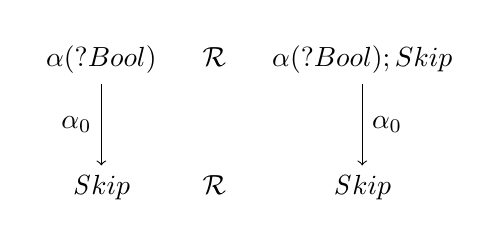
\begin{tikzpicture}
    % Define matrix
        \matrix (m) [matrix of math nodes, row sep=3em, column sep=1em]
        {
            \mathtt\mathit\alpha(?Bool) & \mathcal{R} & \mathtt\mathit\alpha(?Bool);Skip \\
            \mathit Skip & \mathcal{R} & \mathit Skip \\
        };
        % Draw arrows
        \draw[->] (m-1-1) -- (m-2-1) node[midway, left] {$\alpha_0$};
        \draw[->] (m-1-3) -- (m-2-3) node[midway, right] {$\alpha_0$};
    \end{tikzpicture}
\end{center}
    \item $\alpha(?Bool);Skip \xrightarrow{\alpha_1} ?Bool$ via rule \srule{l-varseq2} and type $\alpha(?Bool)$ shares the same transition to $?Bool$ through rule \srule{l-var2}, $\alpha(?Bool) \xrightarrow{\alpha_1} ?Bool$.
    \begin{center}
    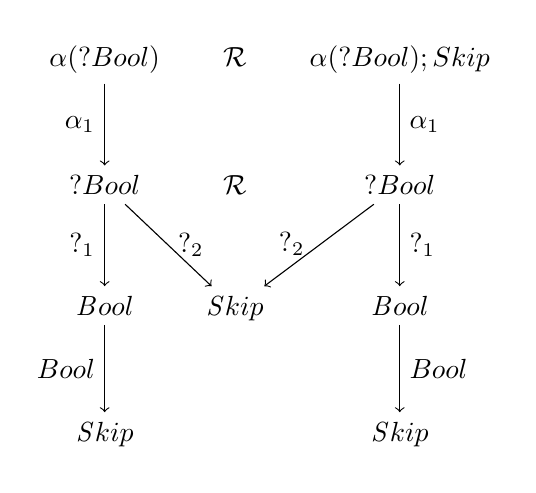
\begin{tikzpicture}
    % Define matrix
        \matrix (m) [matrix of math nodes, row sep=3em, column sep=1em]
        {
            \mathtt\mathit\alpha(?Bool) & \mathcal{R} & \mathtt\mathit\alpha(?Bool);Skip\\
            \mathit ?Bool & \mathcal{R} & \mathit ?Bool \\
            \mathit Bool & \mathit Skip & \mathit Bool \\
            \mathit Skip && \mathit Skip\\
        };
        % Draw arrows
        \draw[->] (m-1-1) -- (m-2-1) node[midway, left] {$\alpha_1$};
        \draw[->] (m-1-3) -- (m-2-3) node[midway, right] {$\alpha_1$};
        \draw[->] (m-2-1) -- (m-3-1) node[midway, left] {$?_1$};
        \draw[->] (m-2-1) -- (m-3-2) node[midway, right] {$?_2$};
        \draw[->] (m-2-3) -- (m-3-3) node[midway, right] {$?_1$};
        \draw[->] (m-2-3) -- (m-3-2) node[near end, above] {$?_2$};
        \draw[->] (m-3-1) -- (m-4-1) node[midway, left] {$Bool$};
        \draw[->] (m-3-3) -- (m-4-3) node[midway, right] {$Bool$};
    \end{tikzpicture}
\end{center}
\end{enumerate} 

There are no transitions with label $Skip$. Therefore, $T\sim U$.\\

\textit{Decidability.   }
Onto the results on decidability of equivalence. 
Following Almeida et al. \cite{AlmeidaMV20}, deciding whether two types are in a type bisimulation takes three steps:

\begin{itemize}
    \item Translating types into simple grammars;
    \item Pruning unreachable symbols;
    \item Exploring a decision tree: two types are equivalent if during this phase we are able to find an empty node; otherwise,
    the types are not equivalent.
\end{itemize}

The first phase is based on Costa et al. \cite{PocasCMV23} function $word(T)$, that translates types to words of nonterminal symbols. This function terminates producing a simple grammar. The notion of simple grammars can be found in section \ref{sec:background}.
After pruning, the type equivalence is decided by the function $bisimG$, introduced by Almeida et al. \cite{AlmeidaMV20}, that checks the bisimilarity of simple grammars.

\section{Programming with $F^{\mu;}_\omega$} \label{sec:term-lang}
In this section, we look at a simple example that takes advantages of $F^{\mu;}_\omega$ types. We use FreeST's syntax freely for the following example.

\begin{lstlisting}
type Stream a = &{Done: Skip, 
                  More: ?a; Stream a}
\end{lstlisting}
Type \lstinline|Stream| offers two choices: \lstinline|Done| which terminates the communication and \lstinline|More|, that reads a value $?a$ and iterates.
This type can be used as a parameter for a fold channel type.

\begin{lstlisting}
type Fold a b =  ?(b $\rightarrow$ a $\rightarrow$ b); ?b;
                    Stream a; !b; Close
\end{lstlisting}
\vspace{3mm}

The type \lstinline|Fold| first receives a folding function followed by the starting element and the elements to fold. We denote the elements we want to fold as a stream, using type \lstinline|Stream|. Then, we send the output of the fold as $!b$ and close the channel.

Let us look at a function that consumes a \lstinline|Fold| channel.

\begin{lstlisting}
foldServer : $\forall$a.$\forall$b. Fold a b $\rightarrow$ $Unit$
foldServer c = 
    let (f,c) = $receive$ c in 
    let (e,c) = $receive$ c in 
    let (r,c) = foldS @a @b f e c in
    c $\vartriangleright$ send r $\vartriangleright$ close
               
foldS : $\forall$a.$\forall$b. (b $\rightarrow$ a $\rightarrow$ b) $\rightarrow$ b 
            $\rightarrow$ Stream a; !b; End 
            $\rightarrow$ (b, !b;Close)
foldS f e (Done c) = (e,c)
foldS f e (More c) = 
    let (x, c) = $receive$ c in
    foldS @a @b f (f e x) c
\end{lstlisting}
\vspace{3mm}
The first function, \lstinline|foldServer|, consumes the first two arguments of the type \lstinline|Fold| channel, that is, receives the folding function and the starting elements, sends the result and terminates the communication by closing the channel. \lstinline|foldS| consumes the stream of elements to fold until the branch $Done$ is selected. Then, we send the pair $(e,c)$, $e$ being the output and $c$ the continuation channel.
Note that $x \vartriangleright f$ stands for the inverse function application, that is $ x \vartriangleright f \vartriangleright g = g (f x)$.

Now we need a client for \lstinline|foldServer|. 

\begin{lstlisting}
type TreeC a = &{Leaf: Skip, 
                 Node: TreeC a; ?a; TreeC a}
\end{lstlisting}
\vspace{3mm}

The type \lstinline|TreeC| offers two choices: $Leaf$ which terminates the communication and $Node$, that receives the left side sub-tree, the root element of that node as $?a$ and the right side sub-tree.
A channel that receives trees in a serialized format would have the following type $TreeChannel\ a = TreeC\ a;Close$.

Next we want to transform our trees from channels to streams. We can write a \lstinline|flatten| function that receives a \lstinline|TreeChannel| and a \lstinline|Stream| and outputs the unused part of the stream.

\begin{lstlisting}
flatten: $\forall$a.$\forall$c. TreeChannel a $\rightarrow$ 
                (Dual Stream a);c $\rightarrow$ c
\end{lstlisting}
\vspace{3mm}

We can finally write our client. This client receives a \lstinline|TreeChannel|, the dual of a \lstinline|Fold| channel and outputs \textbf{\lstinline|True|}, if all the elements in the tree channel are non negative, or false otherwise.

\begin{lstlisting}
allPositive: TreeChannel Int $\rightarrow$
                Dual (Fold Int Bool) 1$\rightarrow$ Bool
allPositive t c = 
    let c = send ($\lambda$x:Bool.$\lambda$y:Int. x 
                    && y > 0 ) c in
    let c = send True c in
    let c = flatten @Int @?Bool;Wait t c in
    let (x,c) = receive c in
    wait c; x
\end{lstlisting}
\vspace{3mm}

First the client sends the folding function, $\lambda x\colon \textbf{\lstinline|Bool|}.\lambda y\colon\textbf{\lstinline|Int|}.\\ 
x\ \&\&\ y\textgreater 0 $, followed by the starting element  \textbf{\lstinline|True|}. Then we call function \lstinline|flatten|. Next, the client receives the output of the \lstinline|Fold| channel, consumes it and waits for the channel to close, $wait c;\ x$.
Note that syntax $flatten\ @Int\ @?Bool;Wait$ stands for term-level type application. 

We can then run both our server and client, like so:
\begin{lstlisting}
main : Bool
main = 
    let tr = forkWith @(TreeC Int) @() 
                produce in
    let fw = forkWith @Dual (Fold Int Bool)
                @() foldServer in
    allPositive tr fw
\end{lstlisting}
\vspace{3mm}

\section{Forthcoming Work and Conclusions} \label{sec:conclusions}

Currently, we are developing test suites for the integration of type operators in FreeST, by using QuickCheck; In particular, we are testing on a small subset of the language, defined by the syntax in section \ref{sec:typeop}. 
It is future work to come up with design solutions for any problems encountered, based on these results, when fully integrating our work into the complete term language of FreeST.\\
The main work scheduled for the following semester is to analyze the current tests, integrate type operators into FreeST, produce new test suites and write the final thesis.\\

To sum up, this paper introduces a type system equipped with equirecursion, abstractions and context-free session types, followed by a type equivalence algorithm all while extending Costa et al. \cite{PocasCMV23} recent work to the programming language FreeST.

%%%%%%%%%%%%%%%%%%%%%%%%%%%%%%%%%%%%%%%%%%%%%%%%%%%%%%%%%%%%%%%%%%%%%%
%% The next two lines define the bibliography style to be used, and
%% the bibliography file.
\bibliographystyle{ACM-Reference-Format}
\bibliography{sample-base}

\end{document}
